% move all configuration stuff into includes file so we can focus on the content
\documentclass[aspectratio=169,hyperref={pdfpagelabels=false,colorlinks=true,linkcolor=white,urlcolor=blue},t]{beamer}

%%%%%%%%%%%%%%%%%%%%%%%%%%%%%%%%%%%%%%%%%%%%%%%%%%%%%%%%%%%%%%%%%%%%%%%%%%%%%%%%%%
%%%%%%%%%%%%%%%%%%%%%%%%%%%%%%%%%%%%%%%%%%%%%%%%%%%%%%%%%%%%%%%%%%%%%%%%%%%%%%%%%%
% packages
\usepackage{pict2e}
\usepackage{epic}
\usepackage{amsmath,amsfonts,amssymb}
\usepackage{units}
\usepackage{fancybox}
\usepackage[absolute,overlay]{textpos} 
\usepackage{media9} % avi2flv: "C:\Program Files\ffmpeg\bin\ffmpeg.exe" -i TuneFreqFilterbank.avi -b 600k -s 441x324 -r 15 -acodec copy TuneFreqFilterbank.flv
\usepackage{animate}
\usepackage{gensymb}
\usepackage{multirow}
\usepackage{silence}
\usepackage[backend=bibtex,style=ieee]{biblatex}
\AtEveryCitekey{\iffootnote{\tiny}{}}
\addbibresource{references}

%%%%%%%%%%%%%%%%%%%%%%%%%%%%%%%%%%%%%%%%%%%%%%%%%%%%%%%%%%%%%%%%%%%%%%%%%%%%%%%%%%
%%%%%%%%%%%%%%%%%%%%%%%%%%%%%%%%%%%%%%%%%%%%%%%%%%%%%%%%%%%%%%%%%%%%%%%%%%%%%%%%%%
% relative paths
\graphicspath{{graph/}}


%%%%%%%%%%%%%%%%%%%%%%%%%%%%%%%%%%%%%%%%%%%%%%%%%%%%%%%%%%%%%%%%%%%%%%%%%%%%%%%%%%
%%%%%%%%%%%%%%%%%%%%%%%%%%%%%%%%%%%%%%%%%%%%%%%%%%%%%%%%%%%%%%%%%%%%%%%%%%%%%%%%%%
% units
\setlength{\unitlength}{1mm}

%%%%%%%%%%%%%%%%%%%%%%%%%%%%%%%%%%%%%%%%%%%%%%%%%%%%%%%%%%%%%%%%%%%%%%%%%%%%%%%%%%
%%%%%%%%%%%%%%%%%%%%%%%%%%%%%%%%%%%%%%%%%%%%%%%%%%%%%%%%%%%%%%%%%%%%%%%%%%%%%%%%%%
% theme & layout
\usetheme{Frankfurt}
\beamertemplatenavigationsymbolsempty
%\setbeamertemplate{frametitle}[smoothbars theme]
\setbeamertemplate{frametitle}
{
    \begin{beamercolorbox}[ht=1.8em,wd=\paperwidth]{frametitle}
        \vspace{-.1em}%
        \hspace{.2em}{\strut\insertframetitle\strut}
        
        \hspace{.2em}\small\strut\insertframesubtitle\strut
        %\hfill
        %
\includegraphics[height=.8cm,keepaspectratio]{CenterMusicTechnology-solid-2lines-white-CoAtag}
        
    \end{beamercolorbox}
    \begin{textblock*}{100mm}(11.6cm,.7cm)
        \includegraphics[height=.8cm,keepaspectratio]{logo_GTCMT_black}
    \end{textblock*}
}

% set this to ensure bulletpoints without subsections
\usepackage{remreset}
\makeatletter
\@removefromreset{subsection}{section}
\makeatother
\setcounter{subsection}{1}

%---------------------------------------------------------------------------------
% appearance
\setbeamercolor{structure}{fg=gtgold}
\setbeamercovered{transparent} %invisible
\setbeamercolor{bibliography entry author}{fg=black}
\setbeamercolor*{bibliography entry title}{fg=black}
\setbeamercolor*{bibliography entry note}{fg=black}

%\usepackage{pgfpages}
%\setbeameroption{show notes}
%\setbeameroption{show notes on second screen=right}
%---------------------------------------------------------------------------------
% fontsize
\let\Tiny=\tiny

%%%%%%%%%%%%%%%%%%%%%%%%%%%%%%%%%%%%%%%%%%%%%%%%%%%%%%%%%%%%%%%%%%%%%%%%%%%%%%%%%%
%%%%%%%%%%%%%%%%%%%%%%%%%%%%%%%%%%%%%%%%%%%%%%%%%%%%%%%%%%%%%%%%%%%%%%%%%%%%%%%%%%
% warnings
\pdfsuppresswarningpagegroup=1
\WarningFilter{biblatex}{Patching footnotes failed}
\WarningFilter{latexfont}{Font shape}
\WarningFilter{latexfont}{Some font shapes}
\WarningFilter{gensymb}{Not defining}


%%%%%%%%%%%%%%%%%%%%%%%%%%%%%%%%%%%%%%%%%%%%%%%%%%%%%%%%%%%%%%%%%%%%%%%%%%%%%%%%%%
%%%%%%%%%%%%%%%%%%%%%%%%%%%%%%%%%%%%%%%%%%%%%%%%%%%%%%%%%%%%%%%%%%%%%%%%%%%%%%%%%%
% title information
\title[]{Introduction to Audio Content Analysis}   
\author[alexander lerch]{alexander lerch} 
%\institute{~}
%\date[Alexander Lerch]{}
\titlegraphic{\vspace{-16mm}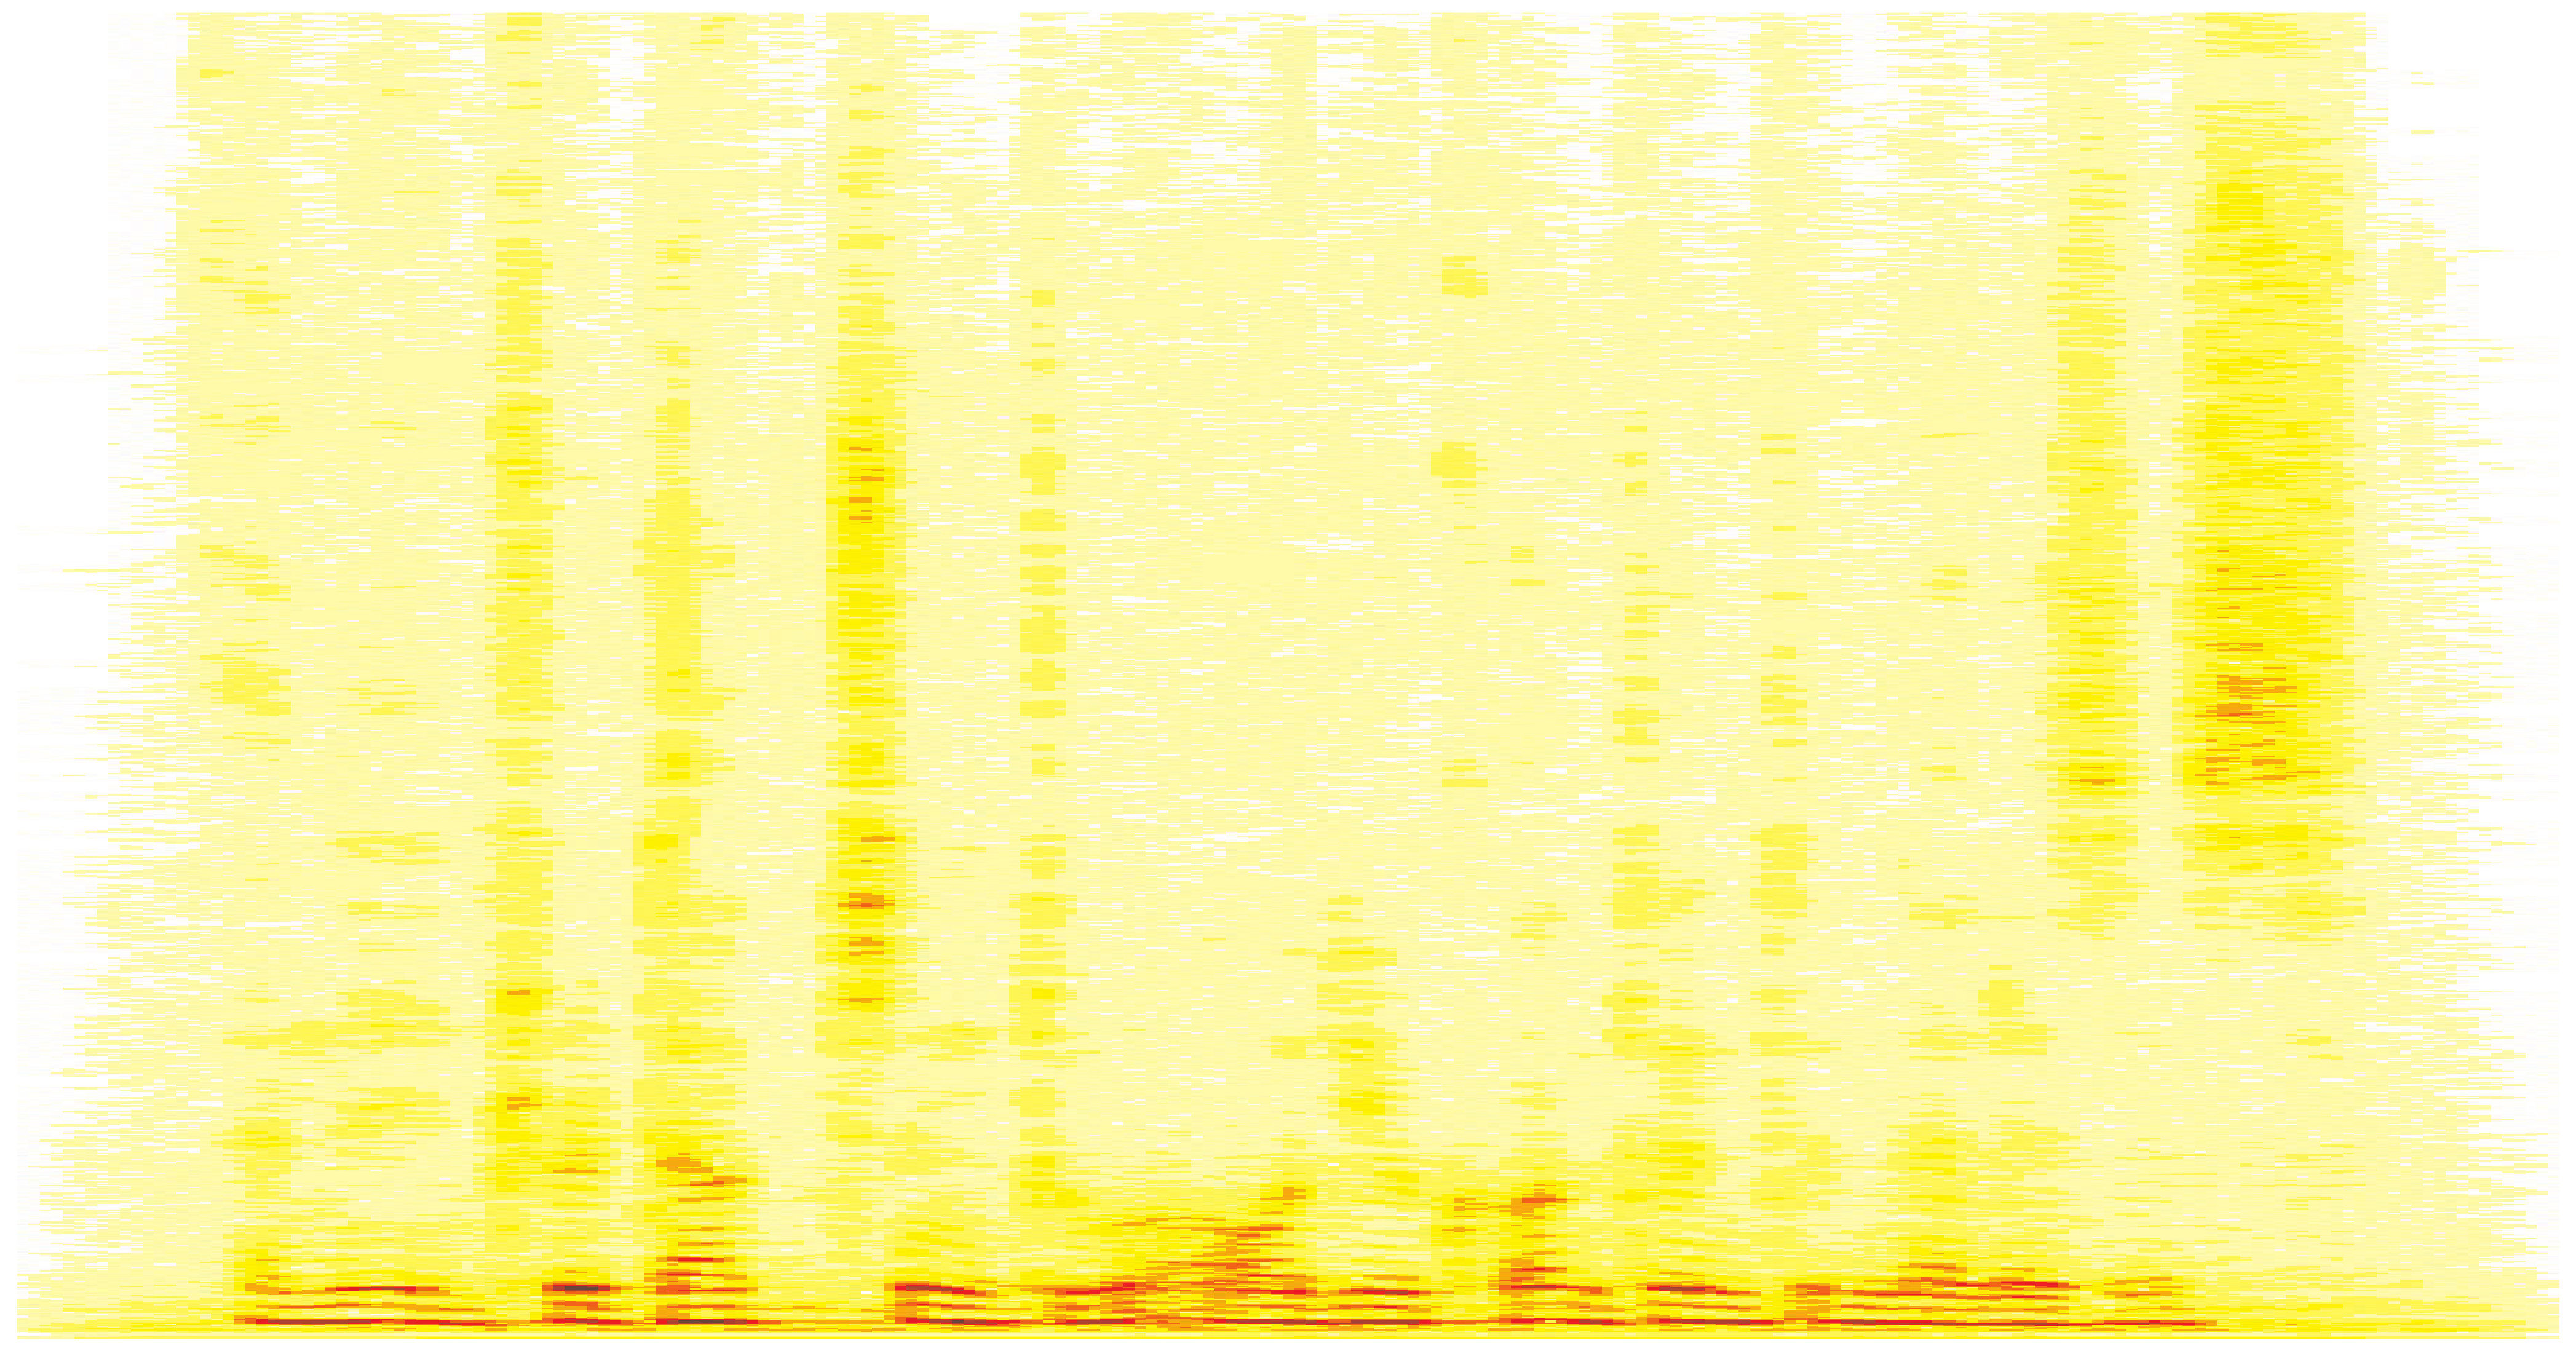
\includegraphics[width=\textwidth,height=3cm]{title}}

%%%%%%%%%%%%%%%%%%%%%%%%%%%%%%%%%%%%%%%%%%%%%%%%%%%%%%%%%%%%%%%%%%%%%%%%%%%%%%%%%%
%%%%%%%%%%%%%%%%%%%%%%%%%%%%%%%%%%%%%%%%%%%%%%%%%%%%%%%%%%%%%%%%%%%%%%%%%%%%%%%%%%
% colors
\definecolor{gtgold}{HTML}{E0AA0F} %{rgb}{0.88,0.66,1,0.06} [234, 170, 0]/256

%%%%%%%%%%%%%%%%%%%%%%%%%%%%%%%%%%%%%%%%%%%%%%%%%%%%%%%%%%%%%%%%%%%%%%%%%%%%%%%%%%
%%%%%%%%%%%%%%%%%%%%%%%%%%%%%%%%%%%%%%%%%%%%%%%%%%%%%%%%%%%%%%%%%%%%%%%%%%%%%%%%%%
% math
\DeclareMathOperator*{\argmax}{argmax}
\DeclareMathOperator*{\argmin}{argmin}
\DeclareMathOperator*{\atan}{atan}
\DeclareMathOperator*{\arcsinh}{arcsinh}
\DeclareMathOperator*{\sign}{sign}
\DeclareMathOperator*{\tcdf}{tcdf}
\DeclareMathOperator*{\si}{sinc}
\DeclareMathOperator*{\princarg}{princarg}
\DeclareMathOperator*{\arccosh}{arccosh}
\DeclareMathOperator*{\hwr}{HWR}
\DeclareMathOperator*{\flip}{flip}
\DeclareMathOperator*{\sinc}{sinc}
\DeclareMathOperator*{\floor}{floor}
\newcommand{\e}{{e}}
\newcommand{\jom}{\mathrm{j}\omega}
\newcommand{\jOm}{\mathrm{j}\Omega}
\newcommand   {\mat}[1]    		{\boldsymbol{\uppercase{#1}}}		%bold
\renewcommand {\vec}[1]    		{\boldsymbol{\lowercase{#1}}}		%bold

%%%%%%%%%%%%%%%%%%%%%%%%%%%%%%%%%%%%%%%%%%%%%%%%%%%%%%%%%%%%%%%%%%%%%%%%%%%%%%%%%%
%%%%%%%%%%%%%%%%%%%%%%%%%%%%%%%%%%%%%%%%%%%%%%%%%%%%%%%%%%%%%%%%%%%%%%%%%%%%%%%%%%
% media9
\newcommand{\includeaudio}[1]{{\includemedia[
                        addresource=audio/#1.mp3,
                        width=5mm,
                        height=5mm,
                        activate=onclick,
                        flashvars={
                            source=audio/#1.mp3  
                            &autoPlay=true
                        }]
                        {
\includegraphics[width=5mm, height=5mm]{SpeakerIcon}}
                        {APlayer.swf}}}
\newcommand{\audioautoplay}[1]{{\begin{center}\includemedia[
                            addresource=audio/#1.mp3,
                            width=.1\linewidth,
                            height=.01\linewidth,
                            activate=pageopen,
                            flashvars={
                                source=audio/#1.mp3  
                                &autoPlay=true
                            }]
                            {}
                            {APlayer.swf}\end{center}}}

\newcommand{\includevideo}[1]{{\begin{center}\includemedia[
                        addresource=video/#1.mp4,
                        width=0.8\linewidth,
                        height=0.4\linewidth,
                        activate=onclick,
                        flashvars={
                            source=video/#1.mp4  
                            &autoPlay=true
                        }]
                        {}
                        {VPlayer.swf}\end{center}}}
\newcommand{\videowithmatlab}[1]{{\begin{center}\includemedia[
                        addresource=video/animate#1.mp4,
                        width=0.8\linewidth,
                        height=0.4\linewidth,
                        activate=onclick,
                        flashvars={
                            source=video/animate#1.mp4  
                            &autoPlay=true
                        }]
                        {}
                        {VPlayer.swf}\end{center}\addreference{matlab source: matlab/animate#1.m}}}
                        

%%%%%%%%%%%%%%%%%%%%%%%%%%%%%%%%%%%%%%%%%%%%%%%%%%%%%%%%%%%%%%%%%%%%%%%%%%%%%%%%%%
%%%%%%%%%%%%%%%%%%%%%%%%%%%%%%%%%%%%%%%%%%%%%%%%%%%%%%%%%%%%%%%%%%%%%%%%%%%%%%%%%%
% other commands
\newcommand{\question}[1]{%\vspace{-4mm}
                          \setbeamercovered{invisible}
                          \begin{columns}[T]
                            \column{.8\textwidth}
                                \textbf{#1}
                            \column{.2\textwidth}
                                \vspace{-8mm}
                                \begin{flushright}
                                     
\includegraphics[scale=.5]{question_mark}
                                \end{flushright}
                                \vspace{6mm}
                          \end{columns}\pause\vspace{-12mm}}

\newcommand{\toremember}[1]{%\vspace{-4mm}
                          \begin{columns}[T]
                            \column{.8\textwidth}
                                \textbf{#1}
                            \column{.2\textwidth}
                                \vspace{-4mm}
                                \begin{flushright}
                                     
\includegraphics[scale=.5]{exclamation_mark}
                                \end{flushright}
                                \vspace{6mm}
                          \end{columns}\vspace{-6mm}}

\newcommand{\matlabexercise}[1]{%\vspace{-4mm}
                          \setbeamercovered{invisible}
                          \begin{columns}[T]
                            \column{.8\textwidth}
                                \textbf{matlab exercise}: #1
                            \column{.2\textwidth}
                                \begin{flushright}
                                     
\includegraphics[scale=.5]{logo_matlab}
                                \end{flushright}
                                %\vspace{6mm}
                          \end{columns}}

\newcommand{\addreference}[1]{  
                  
                    \begin{textblock*}{\baselineskip }(1.12\textwidth,.3\textheight) %(1.15\textwidth,.4\textheight)
                        \rotatebox{90}{\tiny {#1}}
                    \end{textblock*}}
                    
\newcommand{\figwithmatlab}[1]{
                    \begin{figure}
                        \centering
                        \includegraphics{#1}
                        %\label{fig:#1}
                    \end{figure}
                    
                    \addreference{matlab source: \href{https://github.com/alexanderlerch/ACA-Slides/blob/master/matlab/display#1.m}{matlab/display#1.m}}}
\newcommand{\figwithref}[2]{
                    \begin{figure}
                        \centering
                        \includegraphics{#1}
                        \label{fig:#1}
                    \end{figure}
                    
                    \addreference{#2}}  
                                    
\newcommand{\inserticon}[1]{

                    \begin{textblock*}{100mm}(14.5cm,7.5cm)
                        \includegraphics[height=.8cm,keepaspectratio]{#1}
                    \end{textblock*}}            

%%%%%%%%%%%%%%%%%%%%%%%%%%%%%%%%%%%%%%%%%%%%%%%%%%%%%%%%%%%%%%%%%%%%%%%%%%%%%%%%%%
%%%%%%%%%%%%%%%%%%%%%%%%%%%%%%%%%%%%%%%%%%%%%%%%%%%%%%%%%%%%%%%%%%%%%%%%%%%%%%%%%%
% counters
\newcounter{i}
\newcounter{j}
\newcounter{iXOffset}
\newcounter{iYOffset}
\newcounter{iXBlockSize}
\newcounter{iYBlockSize}
\newcounter{iYBlockSizeDiv2}
\newcounter{iDistance}



\subtitle{Module 8.1: Musical Genre Classification}

%%%%%%%%%%%%%%%%%%%%%%%%%%%%%%%%%%%%%%%%%%%%%%%%%%%%%%%%%%%%%%%%%%%%%%%%%%%%
\begin{document}
    % generate title page
	

\begin{frame}
    \titlepage
    %\vspace{-5mm}
    \begin{flushright}
        \href{http://www.gtcmt.gatech.edu}{\includegraphics[height=.8cm,keepaspectratio]{logo_GTCMT_black}}
    \end{flushright}
\end{frame}


    \section[overview]{lecture overview}
        \begin{frame}{introduction}{overview}
            \begin{block}{corresponding textbook section}
                    \href{http://ieeexplore.ieee.org/xpl/articleDetails.jsp?arnumber=6331125}{Chapter 8: Musical Genre, Similarity, and Mood} (pp.~151--155)
            \end{block}

            \begin{itemize}
                \item   \textbf{lecture content}
                    \begin{itemize}
                        \item   musical genre
                        \item   processing steps in basic genre classifiers
                        \item   example: genre classification with a kNN
                    \end{itemize}
                \bigskip
                \item<2->   \textbf{learning objectives}
                    \begin{itemize}
                        \item   discuss ambiguities in the definition of musical genre and the possible impact on automatic systems
                        \item   describe the processing steps for traditional musical genre classifiers
                        \item   implement your own music genre classifier with Matlab
                    \end{itemize}
            \end{itemize}
            \inserticon{directions}
        \end{frame}

    \section[intro]{introduction}
        \begin{frame}{musical genre classification}{introduction}
            \begin{itemize}
                \item	one of the first research topics in MIR
                \item<2->	classic \textit{machine learning }task
                \item<3->	related fields:
                    \begin{itemize}
                        \item	speech-music classification
                        \item	instrument recognition
                        \item   artist identification
                        \item   music emotion recognition
                    \end{itemize}
            \end{itemize}
        \end{frame}

        \begin{frame}{musical genre classification}{applications}
            \begin{itemize}
                \item	large music databases:
                    \begin{itemize}
                        \item	annotation
                        \item	sorting, browsing, retrieving
                    \end{itemize}
                \item recommendation systems
                \item	automatic playlist generation
                \item	mashup generation
            \end{itemize}
        \end{frame}

    \section[genre]{musical genre}
        \begin{frame}{musical genre classification}{genre: definition}
            \question{what is \textit{musical genre}}

            \begin{itemize}
                \item   clusters of musical similarity?
                \item[$\rightarrow$]<2->             hard to answer in general, there are many\\ \textbf{systematic problems}
                \smallskip
                    \begin{enumerate}
                        \item<3->	\textbf{non-agreement on taxonomies}
                        \item<3->   \textbf{genre label scope}: song, album, artist, piece of a song
                        \item<3->	\textbf{ill-defined genre labels}: geographic (\textit{indian music}), historic (\textit{baroque}), technical (\textit{barbershop}), instrumentation (\textit{symphonic music}), usage (\textit{christmas songs})
                        \item<3->	\textbf{taxonomy scalability}: genres and subgenres evolve over time
                        \item<3->	\textbf{non-orthogonality}: several genres for one piece of music
                    \end{enumerate}

            \end{itemize}
            
        \end{frame}
        \begin{frame}{musical genre classification}{genre: taxonomy examples}
                \vspace{-20mm}
                \begin{center}
                \scalebox{.6}
                {
                    				\begin{footnotesize}
					\begin{picture}(150,120)
						%%%%%%%%%%%%%%%%%%%%%%%%%%%%%%%%%%%%%%%%%%%
						%tzanetakis
						\setcounter{iXOffset}{0}
						\put(\value{iXOffset}, 83) {\text{{\shortstack[c]{Speech}}}}
						\put(\value{iXOffset}, 41) {\text{{\shortstack[c]{Music}}}}

						\addtocounter{iXOffset}{10} %10
						\put(\value{iXOffset},49) {\line(1,7){4}}
						\put(\value{iXOffset},48) {\line(1,6){4}}
						\put(\value{iXOffset},47) {\line(1,5){3.5}}
						\put(\value{iXOffset},46) {\line(1,4){3.5}}
						\put(\value{iXOffset},45) {\line(1,3){3.5}}
						\put(\value{iXOffset},44) {\line(1,2){3.5}}
						\put(\value{iXOffset},43) {\line(1,1){3.5}}
						\put(\value{iXOffset},42) {\line(1,-1){3.5}}
						\put(\value{iXOffset},41) {\line(1,-5){3.5}}

						\addtocounter{iXOffset}{1} %11
						\put(\value{iXOffset},85) {\line(1,1){3.5}}
						\put(\value{iXOffset},84) {\line(1,0){3}}
						\put(\value{iXOffset},83) {\line(1,-1){3.5}}
						
						%%%%%%%%%%%%%%%%%%%%%%%%%%%%%%%%%%%%%%%%%%%
						\setcounter{iXOffset}{15}
						\put(\value{iXOffset}, 87) {\text{{\shortstack[c]{Male}}}}
						\put(\value{iXOffset}, 83) {\text{{\shortstack[c]{Female}}}}
						\put(\value{iXOffset}, 79) {\text{{\shortstack[c]{Sports}}}}
						\put(\value{iXOffset}, 75) {\text{{\shortstack[c]{Disco}}}}
						\put(\value{iXOffset}, 71) {\text{{\shortstack[c]{Country}}}}
						\put(\value{iXOffset}, 67) {\text{{\shortstack[c]{Hip Hop}}}}
						\put(\value{iXOffset}, 63) {\text{{\shortstack[c]{Rock}}}}
						\put(\value{iXOffset}, 59) {\text{{\shortstack[c]{Blues}}}}
						\put(\value{iXOffset}, 55) {\text{{\shortstack[c]{Reggae}}}}
						\put(\value{iXOffset}, 51) {\text{{\shortstack[c]{Pop}}}}
						\put(\value{iXOffset}, 47) {\text{{\shortstack[c]{Metal}}}}
						\put(\value{iXOffset}, 37) {\text{{\shortstack[c]{Classical}}}}
						\put(\value{iXOffset}, 17) {\text{{\shortstack[c]{Jazz}}}}
					
						\addtocounter{iXOffset}{8} %28
						\put(\value{iXOffset},20) {\line(1,0.8){8}}
						\put(\value{iXOffset},19) {\line(1,0.5){8}}
						\put(\value{iXOffset},18) {\line(1,0.1){8}}
						\put(\value{iXOffset},17) {\line(1,-0.2){8}}
						\put(\value{iXOffset},16) {\line(1,-0.5){8}}
						\put(\value{iXOffset},15) {\line(1,-0.8){8}}
					
						\addtocounter{iXOffset}{5} %28
						\put(\value{iXOffset},39) {\line(1,1){3.5}}
						\put(\value{iXOffset},38) {\line(1,0.5){3}}
						\put(\value{iXOffset},37) {\line(1,-0.3){3.5}}
						\put(\value{iXOffset},36) {\line(1,-1){3.5}}
					
						%%%%%%%%%%%%%%%%%%%%%%%%%%%%%%%%%%%%%%%%%%%
						\setcounter{iXOffset}{33}
						\put(\value{iXOffset}, 43) {\text{{\shortstack[c]{Choir}}}}
						\put(\value{iXOffset}, 39) {\text{{\shortstack[c]{Orchestra}}}}
						\put(\value{iXOffset}, 35) {\text{{\shortstack[c]{Piano}}}}
						\put(\value{iXOffset}, 31) {\text{{\shortstack[c]{String Quartet}}}}
						\put(\value{iXOffset}, 27) {\text{{\shortstack[c]{Big Band}}}}
						\put(\value{iXOffset}, 23) {\text{{\shortstack[c]{Cool}}}}
						\put(\value{iXOffset}, 19) {\text{{\shortstack[c]{Fusion}}}}
						\put(\value{iXOffset}, 15) {\text{{\shortstack[c]{Piano}}}}
						\put(\value{iXOffset}, 11) {\text{{\shortstack[c]{Quartet}}}}
						\put(\value{iXOffset}, 7) {\text{{\shortstack[c]{Swing}}}}

						%%%%%%%%%%%%%%%%%%%%%%%%%%%%%%%%%%%%%%%%%%%
						%burred
						\setcounter{iXOffset}{80}
						\put(\value{iXOffset}, 71) {\text{{\shortstack[c]{Background}}}}
						\put(\value{iXOffset}, 63) {\text{{\shortstack[c]{Speech}}}}
						\put(\value{iXOffset}, 27) {\text{{\shortstack[c]{Music}}}}

						\addtocounter{iXOffset}{11} 
						
						\put(\value{iXOffset},65) {\line(1,0.4){8}}
						\put(\value{iXOffset},64) {\line(1,0){8}}
						\put(\value{iXOffset},63) {\line(1,-0.4){8}}

						\addtocounter{iXOffset}{-1} 
						
						\put(\value{iXOffset},29) {\line(1,1.3){8}}
						\put(\value{iXOffset},27) {\line(1,-1){8}}
						
						%%%%%%%%%%%%%%%%%%%%%%%%%%%%%%%%%%%%%%%%%%%
						\addtocounter{iXOffset}{10} %100
						\put(\value{iXOffset}, 67) {\text{{\shortstack[c]{Male}}}}
						\put(\value{iXOffset}, 63) {\text{{\shortstack[c]{Female}}}}
						\put(\value{iXOffset}, 59) {\text{{\shortstack[c]{+Background}}}}
						\put(\value{iXOffset}, 42) {\text{{\shortstack[c]{Classical}}}}
						\put(\value{iXOffset}, 16) {\text{{\shortstack[c]{Non-Classical}}}}
						
						\addtocounter{iXOffset}{15} 
						\put(\value{iXOffset},44) {\line(1,1){6}}
						\put(\value{iXOffset},42) {\line(1,-0.8){6}}

						\addtocounter{iXOffset}{5} 
						\put(\value{iXOffset},18) {\line(1,3){2}}
						\put(\value{iXOffset},17) {\line(1,-0.1){2}}
						\put(\value{iXOffset},16) {\line(1,-3){2}}
						
						
						%%%%%%%%%%%%%%%%%%%%%%%%%%%%%%%%%%%%%%%%%%%
						\addtocounter{iXOffset}{3} % 123
						\put(\value{iXOffset}, 49) {\text{{\shortstack[c]{Chamber}}}}
						\put(\value{iXOffset}, 35) {\text{{\shortstack[c]{Orchestra}}}}
						\put(\value{iXOffset}, 25) {\text{{\shortstack[c]{Rock}}}}
						\put(\value{iXOffset}, 15) {\text{{\shortstack[c]{Electro/Pop}}}}
						\put(\value{iXOffset}, 7) {\text{{\shortstack[c]{Jazz/Blues}}}}

						\addtocounter{iXOffset}{8} %131
						\put(\value{iXOffset},27) {\line(1,0.1){10}}
						\put(\value{iXOffset},25) {\line(1,-0.1){10}}

						\addtocounter{iXOffset}{6} %137
						\put(\value{iXOffset},52) {\line(1,0.8){4}}
						\put(\value{iXOffset},51) {\line(1,0.1){4}}
						\put(\value{iXOffset},50) {\line(1,-0.2){4}}
						\put(\value{iXOffset},49) {\line(1,-1){4}}
											
						\addtocounter{iXOffset}{1} %138
						\put(\value{iXOffset},37) {\line(1,0.7){4}}
						\put(\value{iXOffset},36) {\line(1,0){4}}
						\put(\value{iXOffset},35) {\line(1,-0.7){4}}
											
						\addtocounter{iXOffset}{3} %141
						\put(\value{iXOffset},17) {\line(1,1){2}}
						\put(\value{iXOffset},16) {\line(1,0){2}}
						\put(\value{iXOffset},15) {\line(1,-1){2}}
						
						%%%%%%%%%%%%%%%%%%%%%%%%%%%%%%%%%%%%%%%%%%%
						\addtocounter{iXOffset}{3}
						\put(\value{iXOffset}, 55) {\text{{\shortstack[c]{Piano}}}}
						\put(\value{iXOffset}, 51) {\text{{\shortstack[c]{Solo}}}}
						\put(\value{iXOffset}, 47) {\text{{\shortstack[c]{String Quartet}}}}
						\put(\value{iXOffset}, 43) {\text{{\shortstack[c]{Other}}}}
						\put(\value{iXOffset}, 39) {\text{{\shortstack[c]{Symphonic}}}}
						\put(\value{iXOffset}, 35) {\text{{\shortstack[c]{+Choir}}}}
						\put(\value{iXOffset}, 31) {\text{{\shortstack[c]{+Soloist}}}}
						\put(\value{iXOffset}, 27) {\text{{\shortstack[c]{Soft Rock}}}}
						\put(\value{iXOffset}, 23) {\text{{\shortstack[c]{Hard Rock}}}}
						\put(\value{iXOffset}, 19) {\text{{\shortstack[c]{Hip Hop}}}}
						\put(\value{iXOffset}, 15) {\text{{\shortstack[c]{Techno/Dance}}}}
						\put(\value{iXOffset}, 11) {\text{{\shortstack[c]{Pop}}}}
					\end{picture}
				\end{footnotesize}

                }
                \end{center}
        \end{frame}

        \begin{frame}{musical genre classification}{observations with humans}
            \begin{columns}
                \column{.5\linewidth}
                    \begin{enumerate}
                        \item   human classification far from perfect: \unit[75--90]{\%} for limited set of classes
                        \item<2-> for many genres, humans need only a fraction of a second to classify
                        \item<2->[$\Rightarrow$]	short time timbre features sufficient?
                    \end{enumerate}
                \column{.5\linewidth}
                    \begin{figure}
                        \centering
                        \only<1>{
                            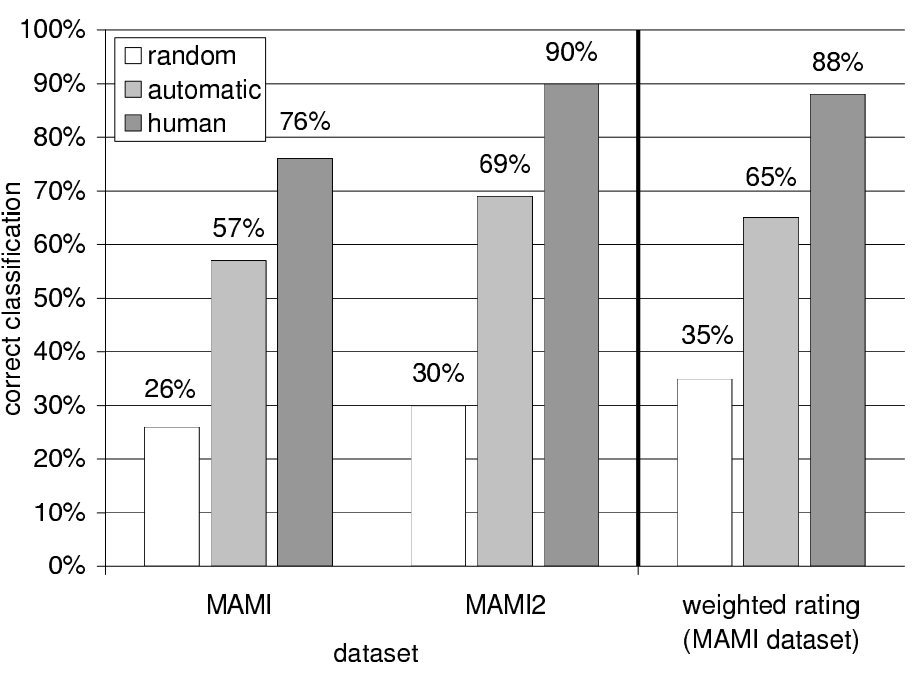
\includegraphics[scale=.2]{graph/genre_human_classification}
                            }
                        \only<2>{
                            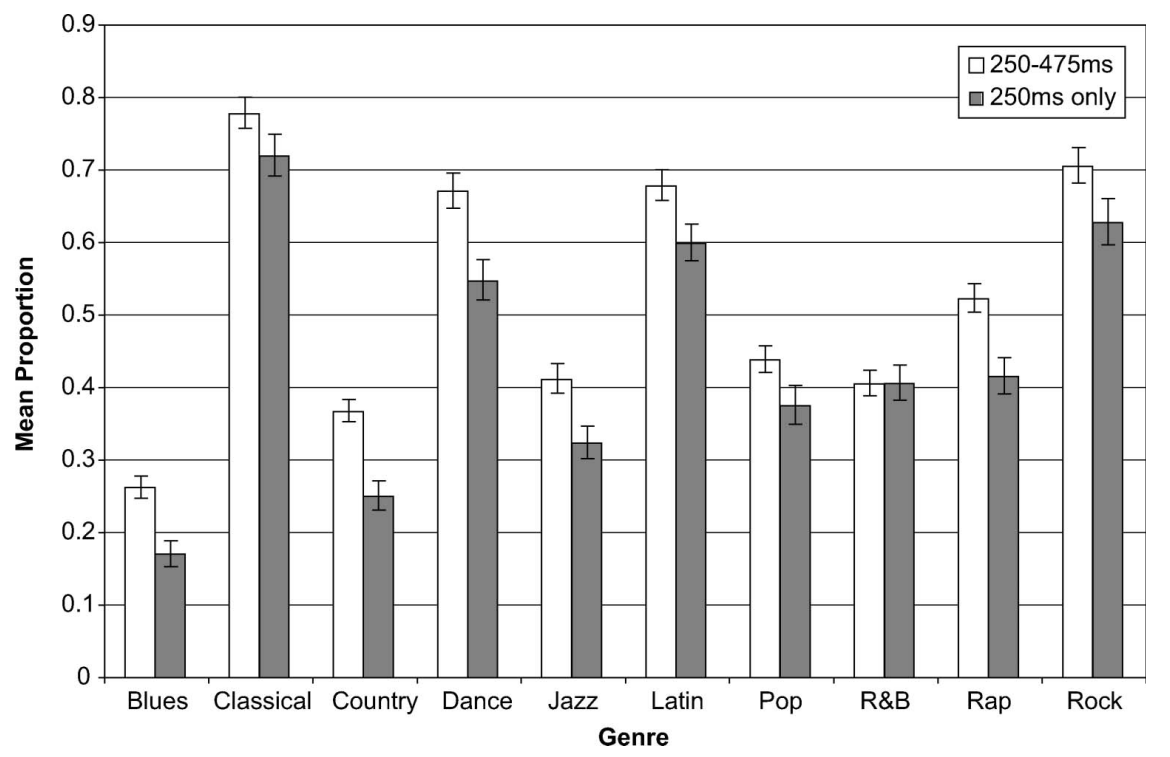
\includegraphics[scale=.15]{graph/genre_shorttime_classification}
                            }
                    \end{figure}
            \end{columns}
            \begin{flushright}plots from \footfullcite{lippens_comparison_2004},\footfullcite{gjerdingen_scanning_2008}\end{flushright}
        \end{frame}
    
    \section[MGC]{automatic musical genre classification}

        \begin{frame}{musical genre classification}{overview}
            \begin{figure}
                \begin{footnotesize}
				\begin{picture}(96,26)
					\setcounter{iXOffset}{0}
					\setcounter{iYOffset}{5}
					\setcounter{iXBlockSize}{28}
					\setcounter{iYBlockSize}{16}
					\setcounter{iYBlockSizeDiv2}{8}
					\setcounter{iDistance}{8}
	
					\addtocounter{iYOffset}{\value{iYBlockSizeDiv2}}
					\addtocounter{iYOffset}{-2}
	
					%\addtocounter{iXOffset}{-1}
					\put(\value{iXOffset}, \value{iYOffset})
						{\text{{\shortstack[c]{Audio\\ Signal}}}}
					\addtocounter{iXOffset}{1}
	
					\addtocounter{iYOffset}{2}
					\addtocounter{iXOffset}{\value{iDistance}}
	
					\put(\value{iXOffset}, \value{iYOffset})
						{\vector(1,0){\value{iDistance}}}
	
					\addtocounter{iXOffset}{\value{iDistance}}
					\addtocounter{iYOffset}{-\value{iYBlockSizeDiv2}}
					
					\put(\value{iXOffset}, \value{iYOffset})
						{\framebox(\value{iXBlockSize}, \value{iYBlockSize}) {{\shortstack[c]{Feature\\ Extraction}}}}
	
					\addtocounter{iXOffset}{\value{iXBlockSize}}
					\addtocounter{iYOffset}{\value{iYBlockSizeDiv2}}
	
					\put(\value{iXOffset}, \value{iYOffset})
						{\vector(1,0){\value{iDistance}}}
	
					\addtocounter{iXOffset}{\value{iDistance}}
					\addtocounter{iYOffset}{-\value{iYBlockSizeDiv2}}
	
					\put(\value{iXOffset}, \value{iYOffset})
						{\framebox(\value{iXBlockSize}, \value{iYBlockSize}) {{\shortstack[c]{Classification}}}}
	
					\addtocounter{iXOffset}{\value{iXBlockSize}}
					\addtocounter{iYOffset}{\value{iYBlockSizeDiv2}}
	
					\put(\value{iXOffset}, \value{iYOffset})
						{\vector(1,0){\value{iDistance}}}
	
					\addtocounter{iXOffset}{\value{iDistance}}
					\addtocounter{iYOffset}{-2}
	
					\addtocounter{iXOffset}{1}
					\put(\value{iXOffset}, \value{iYOffset})
						{\text{{\shortstack[c]{Genre\\ Label}}}}
					
				\end{picture}
\end{footnotesize}
            \end{figure}
            \begin{enumerate}
                    \item	\textbf{feature extraction}
                            \begin{itemize}
                                \item 	dimensionality reduction
                                \item	meaningful representation
                            \end{itemize}
                    \bigskip
                    \item<2->	\textbf{classification}
                            \begin{itemize}
                                \item	map or convert feature to comprehensible domain
                            \end{itemize}
            \end{enumerate}
        \end{frame}

    \section{features}
        \begin{frame}{musical genre classification}{feature categories}
            \vspace{-3mm}
            \begin{itemize}
                \item	\textbf{high level similarities}?
                    \begin{itemize}
                        \item	melody, hook lines, bass lines, harmony progression
                        \item	rhythm \& tempo
                        \item	structure
                        \item	instrumentation \& timbre
                    \end{itemize}
                \smallskip
                \item<2->	\textbf{technical feature categories}
                    \begin{itemize}
                        \item	tonal
                        \item	technical
                        \item	timbral
                        \item	temporal
                        \item	intensity
                    \end{itemize}
                \smallskip
                \item<3->       \textbf{extracted features should be}
                    \begin{itemize}
                        \item   extractable (not: time envelope in polyphonic signals)
                        \item   relevant (not: pitch chroma for instrument ID)
                        \item   non-redundant
                        \item   have discriminative power
                        \item   (robust to noise)
                    \end{itemize}
            \end{itemize}
        \end{frame}

        \begin{frame}{musical genre classification}{instantaneous features}
            \begin{itemize}
                \item	spectral features (\textbf{timbre}):
                
                    Spectral Centroid, MFCCs, Spectral Flux, \ldots
                \smallskip
                \item<2->	pitch features (\textbf{tonal}):
                
                    pitch chroma distribution/change, \ldots
                \smallskip
                \item<3->	rhythm features (\textbf{temporal}):
                
                    onset density, beat histogram features, \ldots
                \smallskip
                \item<4->	statistical features (\textbf{technical}):
                
                    standard deviation, skewness, zero crossings, \ldots
                \smallskip
                \item<5->	\textbf{intensity} features:
                
                    level variation, number of ``pauses'', \ldots
            \end{itemize}	
        \end{frame}

        \begin{frame}{musical genre classification}{feature extraction}
            \begin{enumerate}
                \item	extract \textbf{instantaneous features}
                        \only<1>{
                            \vspace{-5mm}
                            \begin{flushright}
                                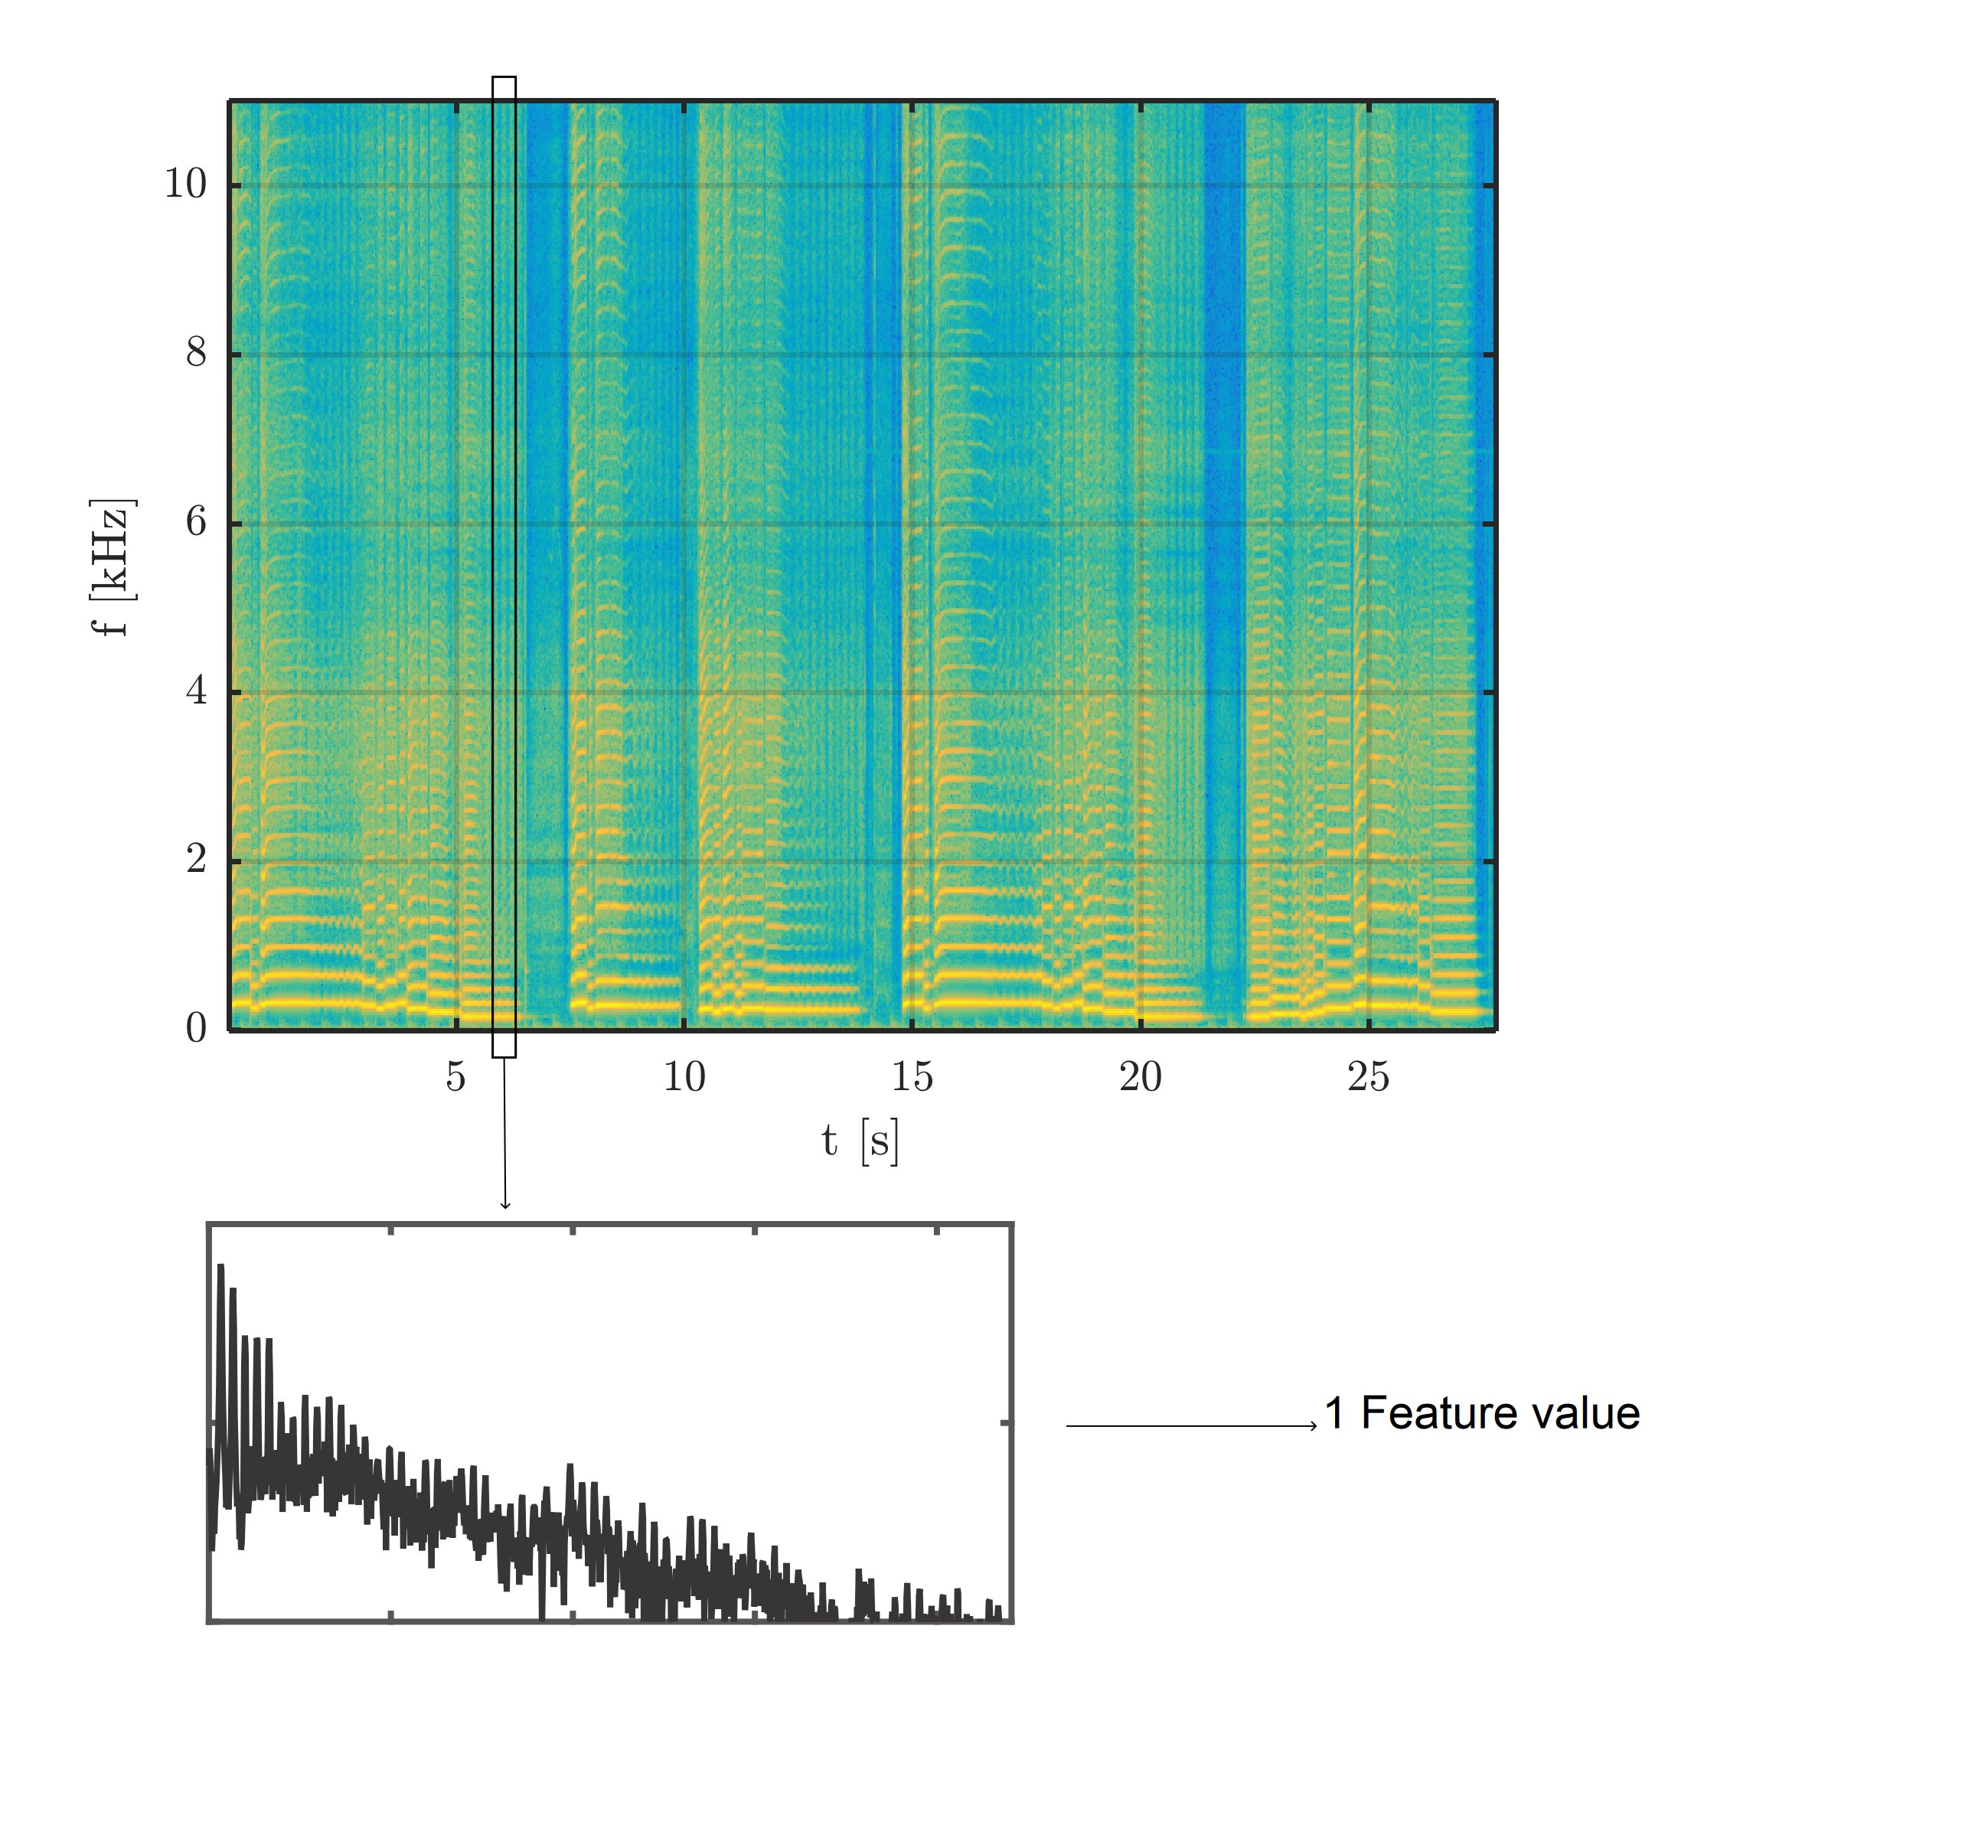
\includegraphics[scale=.05]{graph/FeatureExtraction}
                            \end{flushright}
                            \vspace{-7mm}
                        }
                \smallskip
                \item<2->	compute \textbf{derived features} (derivative, filtered)
                \smallskip
                \item<3->	compute \textbf{long term features} \& subfeatures per texture window
                \smallskip	
                \item<4->	compute \textbf{subfeatures} per file
                \smallskip
                \item<5->   \textbf{normalize} subfeatures
                \smallskip
                \item<6->   (select or) \textbf{transform} subfeatures
                \smallskip
                \item<7->	feature vector $\rightarrow$ \textbf{classifier input}
                            \only<7->{
                            \vspace{-15mm}
                            \begin{flushright}
                                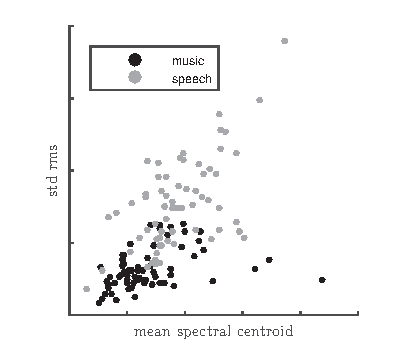
\includegraphics[scale=.7]{graph/Scatter}
                            \end{flushright}
                            }
            \end{enumerate}
            \vspace{20mm}
        \end{frame}
        \begin{frame}{musical genre classification}{long term features 1/2}
            derived from beat histogram\footfullcite{tzanetakis_musical_2002}
            \begin{figure}
                \centering
                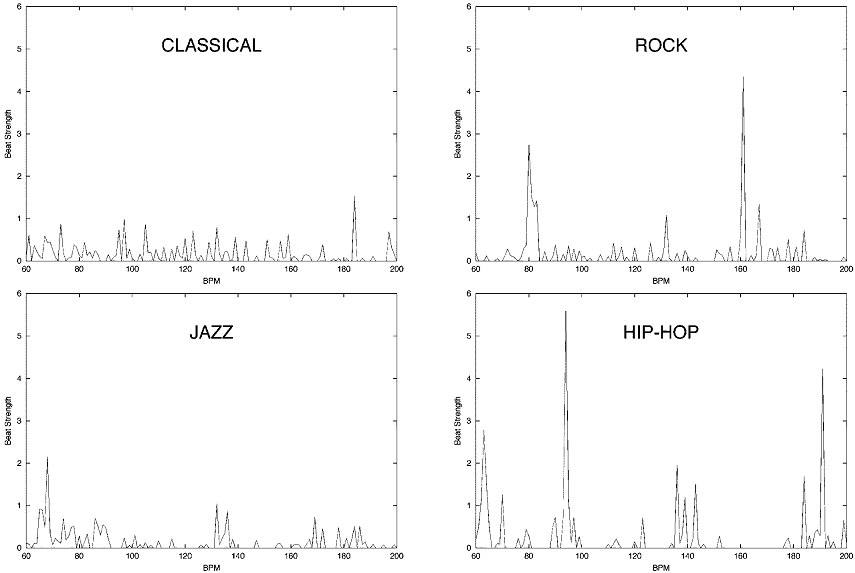
\includegraphics[scale=.25]{graph/genre_beat_histogram}
            \end{figure}
        \end{frame}
        \begin{frame}{musical genre classification}{long term features 2/2}
            derived from pitch histogram or pitch chroma\footfullcite{tzanetakis_pitch_2002}
            \begin{figure}
                \centering
                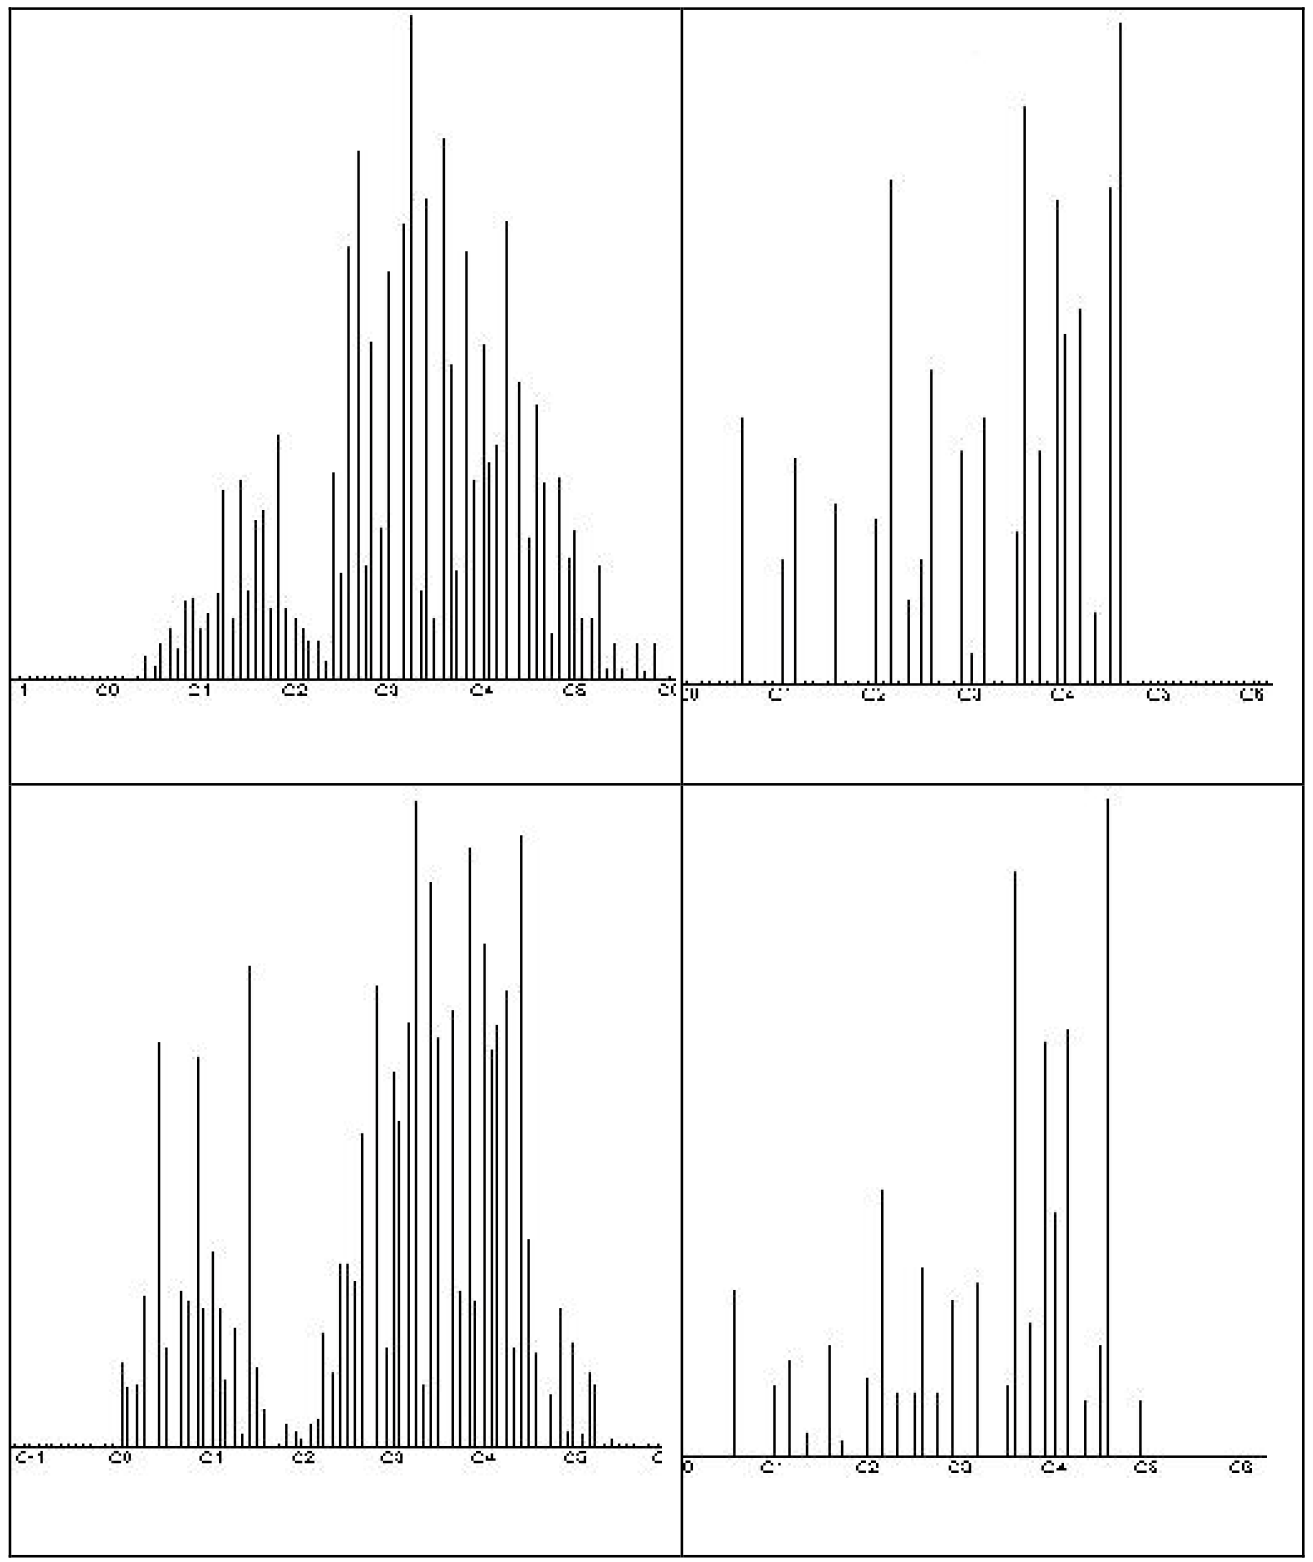
\includegraphics[scale=.12]{graph/genre_pitchhisto}
            \end{figure}
        \end{frame}
        \begin{frame}{musical genre classification}{additional feature examples}
            \begin{itemize}
                \item	\textbf{stereo features}
                    \begin{itemize}
                        \item	mid channel energy vs.\ side channel energy
                        \item	spectral channel differences
                    \end{itemize}
                \bigskip
                \item<2->	features at \textbf{higher semantic levels}:
                    \begin{itemize}
                        \item   tempo, structure, harmonic complexity, instrumentation
                    \end{itemize}
            \end{itemize}
        \end{frame}

        \begin{frame}{musical genre classification}{results}
            \begin{itemize}
                \item	classification results depend on training set, test set, and number of classes
                \smallskip
                \item<2->	typical ranges: 10 classes $\Rightarrow$ 50--80\%
                \smallskip
                \item<3->	note: results vary largely between datasets
                    \begin{itemize}
                        \item   ill-defined genre boundaries
                        \item   non-uniformly distributed classes
                        \item   overfitting through songs from same album or artist
                        \item   \ldots
                    \end{itemize}
            \end{itemize}
        \end{frame}
    \section[example]{real world example}
        \begin{frame}{musical genre classification}{speech/music classification baseline example}
            \begin{enumerate}
                \item	extract features
                \smallskip
                \item   represent each file with its 2-dimensional feature vector
                \smallskip
                \item   kNN to classify unknown audio files
                \smallskip
                \item   evaluate classification performance
            \end{enumerate}
        \end{frame}

        \begin{frame}{musical genre classification}{speech/music classification example: features 1/2}
            for each audio file
            \begin{enumerate}
                \item	split input signal into (overlapping) blocks
                \item	compute 2 feature series (spectral centroid, RMS)
                \item<2->	aggregate feature series to one value each
                    \begin{itemize}
                        \item	\textit{mean} of Spectral Centroid
                            \begin{equation*}
                                \mu_\mathrm{SC} = \frac{1}{N}\sum_{\forall n}{v_\mathrm{SC}(n)}
                            \end{equation*}
                        \item	\textit{standard deviation} of RMS
                            \begin{equation*}
                                \sigma_\mathrm{RMS} = \sqrt{\frac{1}{N}\sum_{\forall n}{(v_\mathrm{RMS}(n)-\mu_\mathrm{RMS})^2}}
                            \end{equation*}
                    \end{itemize}
                \item<3->	represent each file as 2-dimensional vector
                    \begin{equation*}
                        \big(\mu_\mathrm{SC}, \sigma_\mathrm{RMS}\big)^\mathrm{T}
                    \end{equation*}
            \end{enumerate}				
        \end{frame}

        \begin{frame}{musical genre classification}{speech/music classification example: features 2/2}
            \figwithmatlab{Scatter}
        \end{frame}

        \begin{frame}{musical genre classification}{speech/music classification example: training set}
            \begin{itemize}
                \item	use \textbf{dataset} annotated as speech and music:
                    \begin{itemize}
                        \item	requirements
                            \begin{itemize}
                                \item	large compared to number of features
                                \item	representative for use case (diverse)
                            \end{itemize}
                        \item	here (toy example):
                            \begin{itemize}
                                \item	64 speech files
                                \item	64 music files
                            \end{itemize}
                    \end{itemize}
                \bigskip
                \item	extract the features for the dataset
                    \begin{itemize}
                        \item   centroid mean
                        \item   rms std
                    \end{itemize}
                \bigskip
                \item	procedure: Leave-One-Out-Cross-Validation
            \end{itemize}
        \end{frame}

        %\begin{frame}{musical genre classification}{speech/music classification example: evaluation}
            %\begin{itemize}
                %\item 
                    %\textbf{problem}: 
                        %\begin{itemize}
                            %\item   classifier has to be tested with observations \textit{unknown} during training
                            %\item   since annotation is tedious, datasets are often not large enough to split in training and test set
                        %\end{itemize}
                %\bigskip
                %\item<2-> 	\textbf{solution}: \textit{N-Fold Cross Validation}
                    %\begin{enumerate}
                        %\item	split training set into $N$ parts (randomly, but identical number per class)
                        %\item<3->	select one part as test set
                        %\item<4->	train the classifier with all observations from \textit{remaining} $N-1$ parts
                        %\item<5->	compute the classification rate for the \textit{test set}
                        %\item<6->	repeat until all $N$ parts have been tested
                        %\item<7->	overall result: \textit{average} classification rate
                    %\end{enumerate}
            %\end{itemize}
        %\end{frame}

        \begin{frame}{musical genre classification}{speech/music classification example: results (kNN)}
            \begin{itemize}
                \item   \textbf{confusion matrix}:
                    \begin{table}
                        \centering
                        \begin{tabular}{l|cc|ccccccccc} %{\textwidth}{@{\extracolsep{\fill}}ccccccccccccc}
                            \bf{\emph{}}	 & \bf{\emph{speech}}	 & \bf{\emph{music}} & \# files	 \\ 
                             \hline
                            \bf{speech}	 & $\mathbf{53}$	 & $11$	 & $64$\\
                            \bf{music}	 & $10$	 & $\mathbf{54}$ & $64$
                        \end{tabular}
                    \end{table}
                \item<2->$\Rightarrow$ \textbf{classification rate}: 
                    \begin{equation*}
                        \frac{53 + 54}{64 + 64} = 83.59\%
                    \end{equation*}
                \smallskip
                \item<3->   single feature classification results
                    \begin{itemize}
                        \item	Spectral Centroid: $64.84\%$
                        \item	RMS: $76.56\%$
                    \end{itemize}
            \end{itemize}
            \addreference{matlab source: \href{https://github.com/alexanderlerch/ACA-Slides/blob/master/matlab/computeMusicSpeechClassification.m}{matlab/computeMusicSpeechClassification.m}}
                        
        \end{frame}
    
    \section{summary}
        \begin{frame}{summary}{lecture content}
            \begin{itemize}
                \item   \textbf{musical genre}
                    \begin{itemize}
                        \item   ill-defined, subjective, no general agreement
                    \end{itemize}
                \bigskip
                \item   \textbf{MGC: features}
                    \begin{enumerate}
                        \item   from all possible categories as all categories might depend on genre
                    \end{enumerate}
                \bigskip
                \item   \textbf{MGC: classifier}
                    \begin{enumerate}
                        \item   any classifier is good, and most have been used
                    \end{enumerate}
            \end{itemize}
            \inserticon{summary}
        \end{frame}
\end{document}
